\subsection{What is skew and what does it measure? }

\cite{das1998smiles} have eloquently answered this question in the introduction of the paper. As per the theoretical framework of Black and Scholes, the implied volatility is independent of the strike price for a given expiration, since the implied volatility is an input parameter to the model used to price the option. As per \cite{das1998smiles}, the volatility smile stems from the presence of excess kurtosis in the conditional returns distribution and an asymmetry in the volatility smile is due to the skewness in this distribution.

Another study by \cite{mixon2011volatility} provides an extensive literature review for different measures of skew in options markets. The paper identifies that the ad hoc measures of skewness lack a rigorous justification because they do not control for volatility and kurtosis implicit in the distribution. The author presents the normalised difference between a 25-Delta put and a 25-Delta call which he argues to be the least redundant among the other competitor metrics that he analysed. The measure of skewness that we have used in this paper is directly taken from \cite{mixon2011volatility}, which is:
$$ \text{Skew} = \frac{IV_\text{25D-Put} - IV_\text{25D-Call}}{IV_\text{50D-Put} } $$

However, for now, I will keep it very simple. The skew is calculated as the difference between the implied volatility of 25-Delta call and 50-Delta Call.
$$ \text{Skew} = \frac{IV_\text{25D-Call}} {IV_\text{50D-Call}}$$



\textit{Note to instructor, to be removed later: Right now I just wanted to see how the skew looks like. A proper measure of skew would require a bit more careful and involved work as I would need to join the call option contracts with their counterpart put options contracts.}


The distribution of skew looks very similar to the the distribution of the OTM implied volatility. It is characterized by very long tails and a high variability especially for the interest rate dependent tickers. 


\begin{figure}[H]
    \centering
    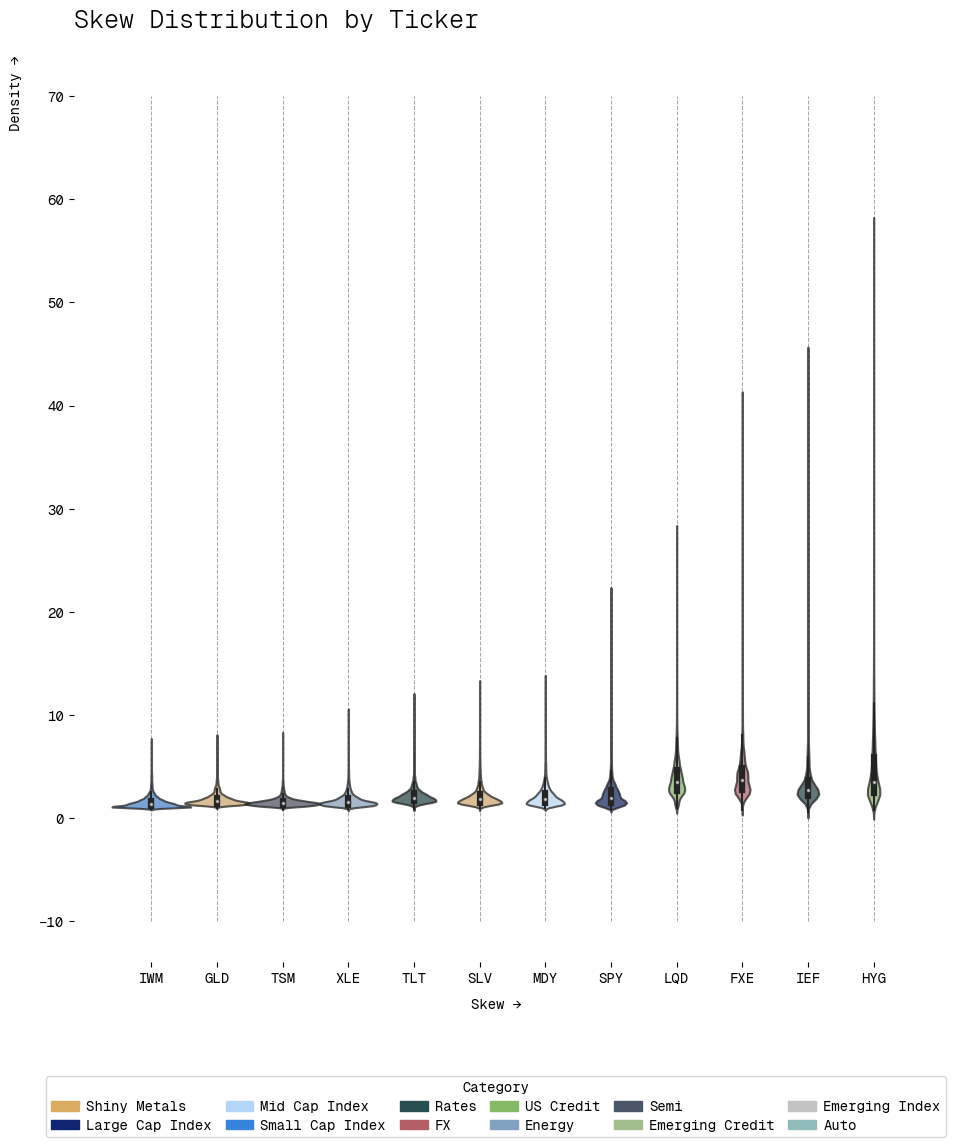
\includegraphics[width=1\textwidth]{images/skew_violin.png}
    \caption{Distribution of Skew}
    \label{fig:skew_violin}
\end{figure}

The relationship of skew is also similar to those of OTM IVs that is a cone like shape for almost every ticker. The interpretation is that when the realised volatility is low the skew clustered at the lower end in a narrow area. As the uncertainty increases, the range of skews that are observed becomes wide.

\begin{figure}[H]
    \centering
    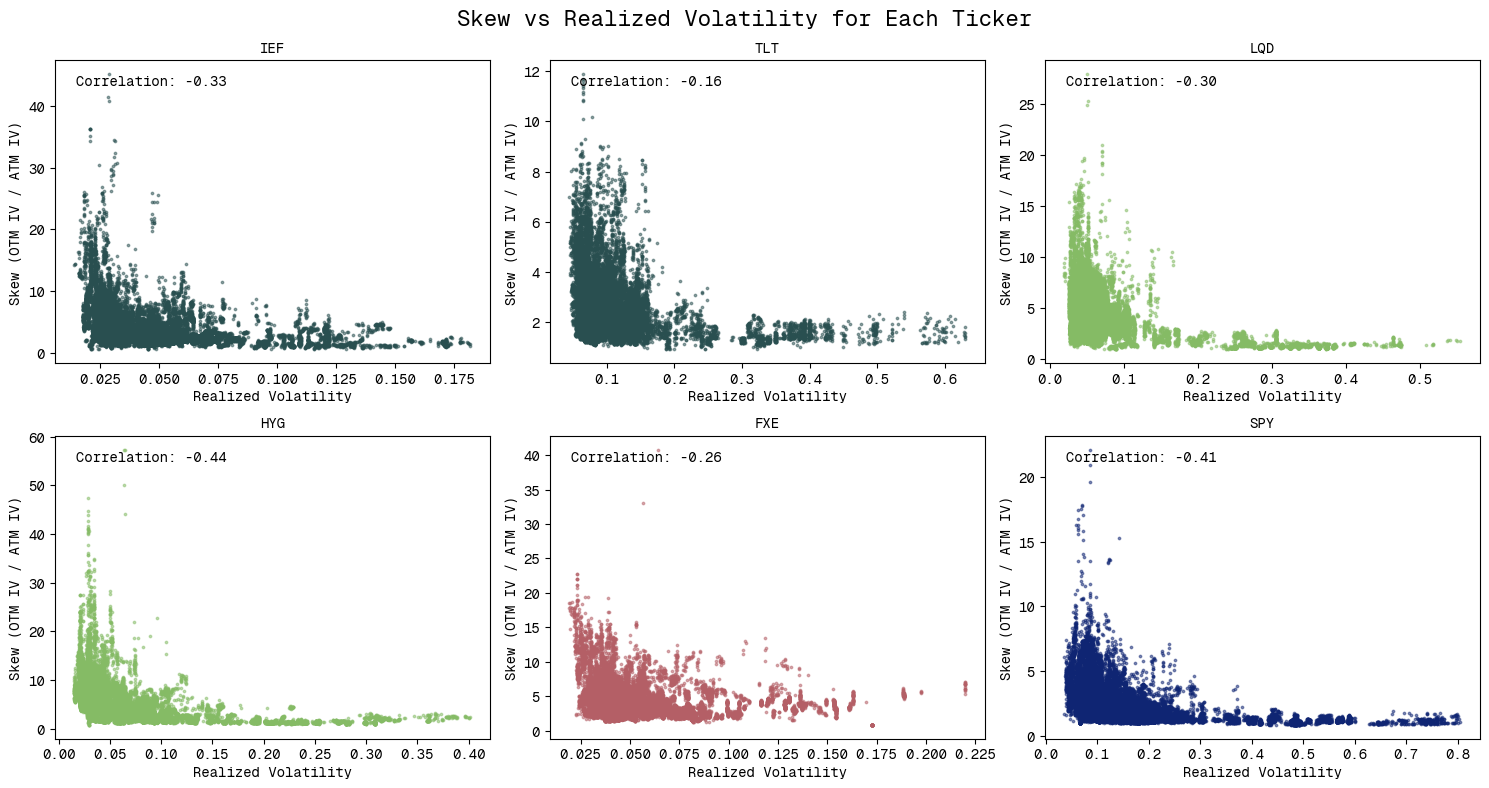
\includegraphics[width=1\textwidth]{images/skew_and_rv_otm_batch1.png}
    \caption{Distribution of Skew}
    \label{fig:skew_and_rv_otm_batch1}

    
\end{figure}
    \begin{figure}[H]
        \centering
        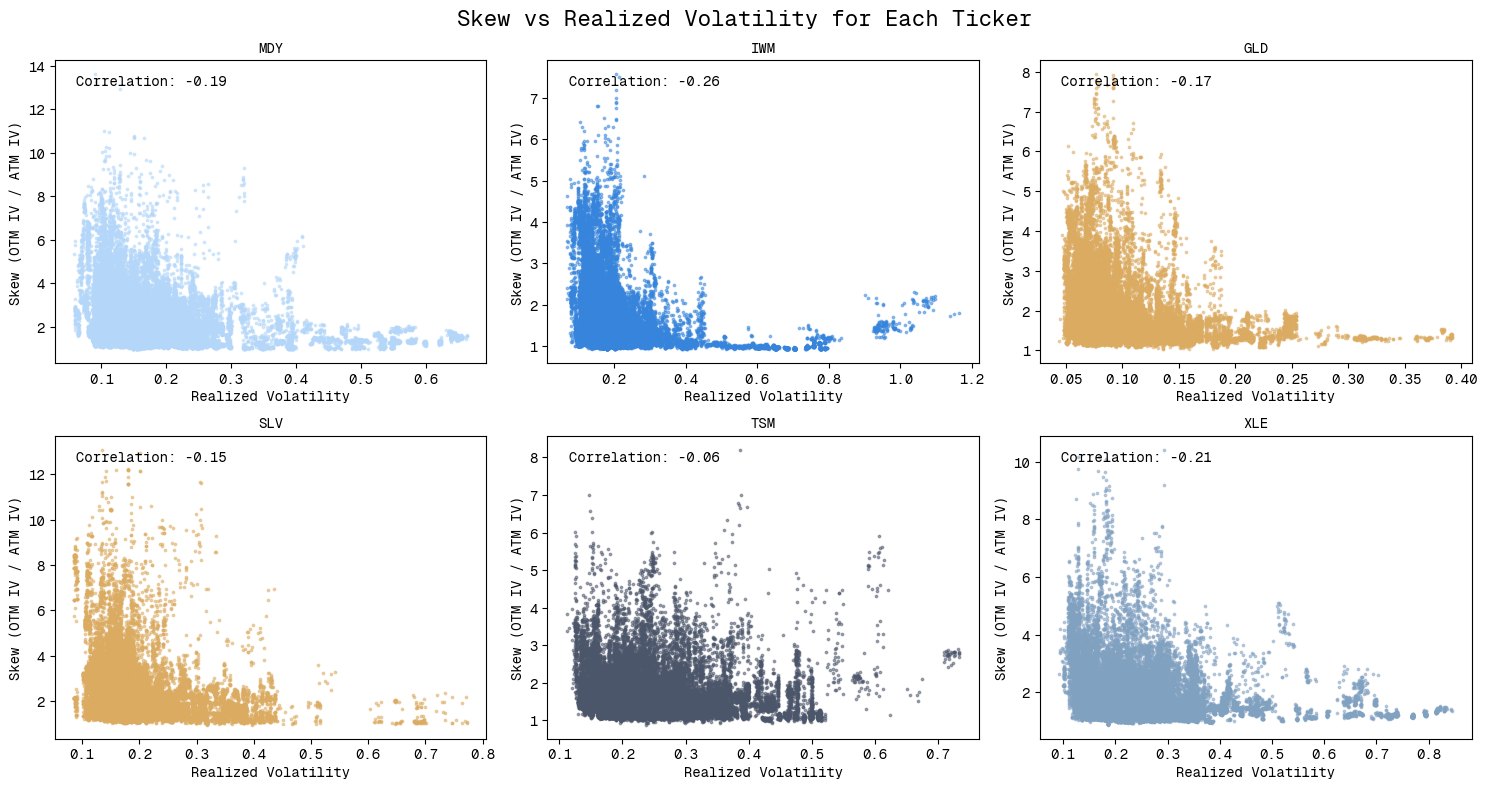
\includegraphics[width=1\textwidth]{images/skew_and_rv_otm_batch2.png}
        \caption{Distribution of Skew}
        \label{fig:skew_and_rv_otm_batch2}
    \end{figure}
